\documentclass{beamer}
\usepackage[british,spanish]{babel}
\usepackage[utf8]{inputenc}
\usepackage{hyperref}
\usepackage{multirow}



\usepackage{listings}

\usepackage{adjustbox}
\usepackage{lstcustom}

\usepackage{color}
\definecolor{light-gray}{gray}{0.80}
\definecolor{lstbackgroundshellcolor}{named}{light-gray}

\usepackage{tikz}
\newcommand*\circled[1]{\tikz[baseline=(char.base)]{
            \node[shape=circle,draw,inner sep=2pt] (char) {#1};}}

\usepackage[normalem]{ulem}

%\usepackage[acronym,xindy,toc]{glossaries}

\usepackage[acronym,xindy,toc]{glossaries}
\makeglossaries
%\usepackage[xindy]{imakeidx}
%\makeindex

\newcommand{\comment}[2]{#2}

\graphicspath{ {./images/} }

\title[Cloud Computing with Amazon Web Services]{Cloud Computing with Amazon Web Services}
%\subtitle[short subtitle]{long subtitle}
\author[C. Cuenca, F. Quintana]{Carmelo Cuenca-Hernández and Francisca Quintana-Domínguez}
%\institute{Escuela Universitaria de Informática}
%\date[04/2013]{Abril - 2013}
\date{}
\titlegraphic{
\includegraphics[width=0.5 \textwidth]{images/awslogo.eps}}



\pgfdeclareimage[width=2.0\baselineskip]{ulpgc-logo}{images/logosimbolo_secundario_version_vertical}
\setbeamertemplate{footline}{\raisebox{-2ex}{\pgfuseimage{ulpgc-logo}}
  \usebeamerfont{date in head/foot}\insertshortdate{}\hfill
  \usebeamertemplate{navigation symbols}\hfill
  \insertframenumber{}/\inserttotalframenumber}
\setbeamertemplate{sidebar right}{}


\usetheme{Antibes}
%\usetheme{Berlin}

%\usetheme{Warsaw}
%\usecolortheme{albatross}

\begin{document}

\begin{frame}
	\titlepage
\end{frame}


\section*{Outline}
\begin{frame}
  \frametitle{Outline}
  %\tableofcontents%[part=1,pausesections]
  %\tableofcontents[currentsection,currentsubsection, sectionstyle=show] 
  \tableofcontents[currentsection,sectionstyle=show,hideothersubsections]
\end{frame}


\selectlanguage{british}

%%%%%%%%%%%%%%%%%%%%%%%%%%%%%%%%%%%%%%%%%%%%%%%%%%%%%%%%%%%%%%%%%%%%%%%%%%%%%%
%\newacronym{<label>}{<abbrv>}{<full>}
%\glsreset{<label>}
%\glsresetall
%\acrlong{<label>}
%\acrfull{<label>}
%\acrshort{<label>}
\newacronym{aws}{AWS}{Amazon Web Services}
\newacronym{ebs}{EBS}{Elastic Block Storage}
\newacronym{ec2}{EC2}{Amazon Elastic Compute Cloud}
\newacronym{ecu}{ECU}{Elastic Compute Unit}
\newacronym{elb}{ELB}{Elastic Load Balancing}
\newacronym{rds}{RDS}{Relational Database Service}
\newacronym{s3}{S3}{Simple Storage Service}
\newacronym{sqs}{SQS}{Amazon Simple Queue Service}
%%%%%%%%%%%%%%%%%%%%%%%%%%%%%%%%%%%%%%%%%%%%%%%%%%%%%%%%%%%%%%%%%%%%%%%%%%%%%%
\section[Amazon Web Services]{Amazon Web Services}
\section{Sign Up Amaon Web Service}
%%%%%%%%%%%%%%%%%%%%%%%%%%%%%%%%%%%%%%%%%%%%%%%%%%%%%%%%%%%%%%%%%%%%%%%%%%%%%%
\begin{frame}
\frametitle{Amazon Web Services}
\begin{figure}
  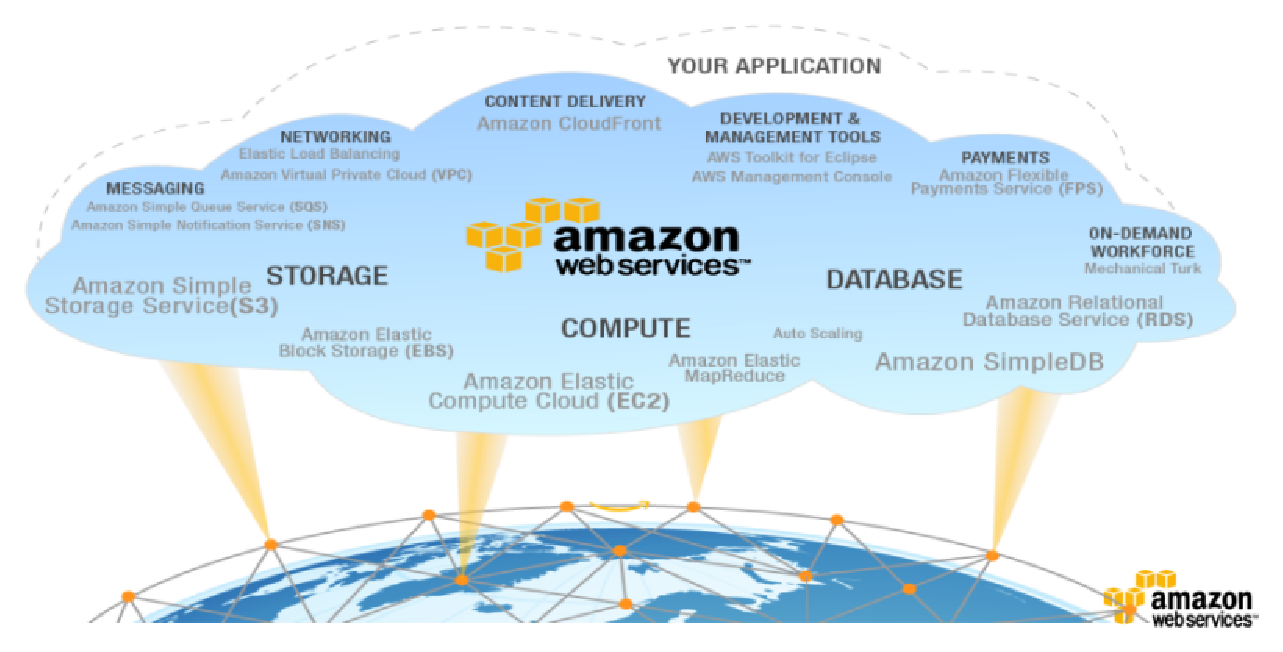
\includegraphics[width= 1.0 \textwidth]{infraestructura-tecnologica-de-amazon-web-services-para-brindar-servicios-cloud-saas-iaas-y-paas.eps}
\end{figure}
\end{frame}
%%%%%%%%%%%%%%%%%%%%%%%%%%%%%%%%%%%%%%%%%%%%%%%%%%%%%%%%%%%%%%%%%%%%%%%%%%%%%%
%%%%%%%%%%%%%%%%%%%%%%%%%%%%%%%%%%%%%%%%%%%%%%%%%%%%%%%%%%%%%%%%%%%%%%%%%%%%%%
\begin{frame}[fragile]
\frametitle{Registration in Amazon Web Services}
\begin{itemize}
 \item All you need \dots
 \begin{itemize}
   \item A desktop or laptop (with Internet access, of course)
   \item A credit card (for setting up an AWS account)
   \item A phone (to complete the registration process)
 \end{itemize}
\end{itemize}
\end{frame}
%%%%%%%%%%%%%%%%%%%%%%%%%%%%%%%%%%%%%%%%%%%%%%%%%%%%%%%%%%%%%%%%%%%%%%%%%%%%%%
%%%%%%%%%%%%%%%%%%%%%%%%%%%%%%%%%%%%%%%%%%%%%%%%%%%%%%%%%%%%%%%%%%%%%%%%%%%%%%
\begin{frame}[fragile, allowframebreaks]
\frametitle{Registration in Amazon Web Services}
\begin{itemize}
\item Choose \texttt{Sign Up} button in \url{http://aws.amazon.com/console/} 
\begin{enumerate}
 \item  Create an AWS Account: Login Credentials and Contact Information
  \item Payment Method: Credit Card, Card Number, Cardholder's Name, Expiration Date, Value Added Tax Information
  \item Identity Verification
  \item Support Plan
 \end{enumerate}

\item Sign in!
\item Navigate to Billing and Cost Management, then Credits an introduce de Promotional Code
\begin{center}
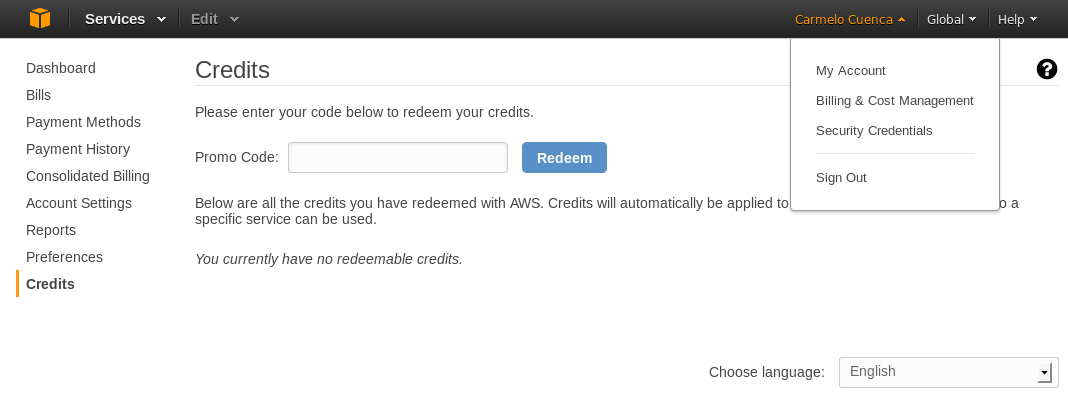
\includegraphics[scale=0.25]{credits.png}
\end{center}
\end{itemize}

\end{frame}
%%%%%%%%%%%%%%%%%%%%%%%%%%%%%%%%%%%%%%%%%%%%%%%%%%%%%%%%%%%%%%%%%%%%%%%%%%%%%%
%%%%%%%%%%%%%%%%%%%%%%%%%%%%%%%%%%%%%%%%%%%%%%%%%%%%%%%%%%%%%%%%%%%%%%%%%%%%%%


\end{document}

